% Chapter 1

\chapter{Results and Analysis} % Main chapter title

\label{Chapter5} % For referencing the chapter elsewhere, use \ref{Chapter1} 

\lhead{Chapter 5. \emph{Results and Analysis}} % This is for the header on each page - perhaps a shortened title

\emph{This chapter presents the results of our implementation work, which comprises of 66 cross-validated feature engineering experiments including a baseline evaluation. It notably begins with a comparison between GROBID and refextract, the existing partial solution for metadata extraction within INSPIRE-HEP. Following this, the evaluation method and approach to running experiments are detailed. Finally, the experimental results are presented and we provide our analysis and interpretations. The results are first shown by category, in accordance with the methods described in Chapter \ref{Chapter4}, then inter-category results are shown to highlight the most significant improvements.}

\section{Evaluation Method}

Cross-validation (see Section \ref{sec:experimentsetup}) is use to give an estimation of model generalisation error. When it comes to reporting results, we focus on the cross-validated performance metric, micro average (see Section \ref{subsec:evaluationmethod}). This is more informative than a \emph{macro} average due to the skew in class representation. For example, the <abstract> class contains on average far more tokens than any other class in the \emph{header} model; likewise, <body> for \emph{segmentation}. The micro average effectively gives a weighted average that says more about general token accuracy. Where necessary, we further look at model performance in individual fields. For the \emph{segmentation} model, the key fields are <header> and <references>. For the \emph{header} model, they are <title>, <authors>, and <abstract>.

\subsection{Evaluation Metrics}
\label{subsec:evaluationmethod}

The findings of this chapter refer to various standard measures of classification performance. We define these presently. Accuracy is defined to be,

\begin{equation}
\text{Accuracy} = \frac{TP + TN}{TP + FN + FP + TN},
\label{eq:accuracy}
\end{equation}

that is, the proportion of correct classifications to total classifications, where TP is the number of \emph{true positives}, the number of times a class is correctly predicted to have occurred; TN is the number of \emph{true negatives}, the number of times a given class is correctly predicted not to have occurred; FN is the number of \emph{false negatives}, the number of times a class is incorrectly predicted to have occurred; and FN is the number of \emph{false negatives}, the number of times a class is incorrectly predicted not to have occurred. Accuracy can be a misleading statistic when we have uneven representations of classes in the dataset. In the event that we have a sufficiently high bias, we can achieve excellent accuracy simply by always predicting the dominant class. For this reason, we consider other statistics too. \emph{Precision} is the number of times a class is \emph{correctly} predicted proportional to the overall number of predictions for that class, that is,

\begin{equation}
\text{Precision} = \frac{TP}{TP + FP}.
\label{eq:precision}
\end{equation}

This, however, does not inform us as to whether we have missed any occurrences of the class, which would be shown in the number of false negatives, FN. We could therefore have a very high precision with limited accuracy. \emph{Recall} is the number of times a class is \emph{correctly} predicted proportional to the number of occurrences of that class (equivalently, the accuracy with respect to the class), that is,

\begin{equation}
\text{Recall} = \frac{TP}{TP + FN}.
\label{eq:recall}
\end{equation}

However, a simple strategy of always predicting one class will give perfect recall for that class, because then misclassifications are only captured by $FP$. The $F_1$ statistic is a common measure used to assess classifiers that combines precision and recall, and is defined as,

\begin{equation}
F_1 = \frac{2 \times \text{precision} \times \text{recall}}{\text{precision} + \text{recall}},
\label{eq:f1}
\end{equation}

that is, the harmonic mean of precision and recall (the ``1'' in $F_1$ indicates the two are evenly weighted). The $F_1$ statistic is a neat way of summarising both metrics at once. Furthermore, a large imbalance in precision and recall results in a lower $F_1$ score. It is necessary to be good in both precision and recall to have a good $F_1$ score; the harmonic mean of any data is always upper-bounded by its arithmetic mean. Thus, the $F_1$ score addresses their shortcomings simultaneously. To summarise each of these statistics over a set of classes, we may adopt two approaches: macro and micro averages. A macro average is the aggregation of statistics \emph{a posteriori}. For example, for accuracy,

\begin{equation}
\text{Accuracy}_{macro} = \frac{1}{N}\sum_{n=1}^{N}\text{Accuracy}_n,
\label{eq:macroaccuracy}
\end{equation}

where $\text{Accuracy}_n$ is the accuracy for the $nth$ of $N$ classes. By contrast, a micro average is an aggregation of statistics that is in effect weighted by the proportion of each class. For example, again for accuracy,

\begin{equation}
\text{Accuracy}_{micro} = \frac{\sum_{n=1}^N TP_n + TN_n}{\sum_{n=1}^N TP_n + FP_n + FN_n + TN_n},
\label{eq:microaccuracy}
\end{equation}

\subsection{Evaluation in GROBID}

GROBID calculates the aforementioned statistics for each of the classes in each model. In our results (Section \ref{sec:results}), we concentrate on the $F_1$ score micro average and scores for key classes (depending on the model we consider) at the \emph{token} level. We supplement the GROBID evaluation output with our own confusion matrices, an example of which is shown in Figure \ref{fig:segmentation_baseline_confusion}. Whereas the metrics allow us to compare one model to another, a confusion matrix can be used to see exactly which misclassifications are being made, which can in turn inform our feature engineering.

\section{Experiment Setup}
\label{sec:experimentsetup}

Our computing resources for experimentation consisted of two powerful virtual machines on the CERN LXPLUS cluster, each possessing 16 CPUs and 32 GB of RAM. The experiments were configured and uploaded to these machines in batches, and were processed by our experimentation pipeline (see Section \ref{subsec:pipeline}). The high dimensionality of the models (up to tens of millions of features) led to long runtimes. To control the runtime of training, we enforced a maximum number of 500 iterations for Wapiti's L-BFGS algorithm. This number was chosen from observing the diminishing improvements of models trained to this extent\footnote{There is also the argument that training to convergence may cause overfitting.}. With Wapiti parallelised to 8 cores, we were able to run two processes on each virtual machine when required. Even with this parallelised setup, our experiment batches took several days to process each time, and the sum total of our experiments amounts to perhaps months of CPU time. Recall that model training time is dependent on both the number of training samples and the model dimensionality, which is itself dependent on the number of samples (see Section \ref{sec:lbfgs}).

In conjunction with our feature engineering variations, we tried different configurations of data. Figure \ref{fig:cv} illustrates our four approaches to cross-validation with different combinations of HEP and CORA training data. Where we \emph{append} data, we include it in training, but exclude it from evaluation. Thus, HEP app. CORA denotes the training of a model on HEP and CORA combined, but cross-validation and evaluation only on HEP. Of most interest, naturally, were those configurations evaluating purely on HEP papers, that is, those we denote \emph{HEP} and {HEP app. CORA}, and these were the only configurations run beyond the baseline. In Section \ref{sec:results}, we refer to these configurations as we present the results. All experiments were run with $5-$fold cross validation\footnote{Note that by a happy coincidence this allows us to read individual CV iteration results from our boxplots as they correspond directly with $Q_1$, $Q_2$, $Q_3$, and the two outliers (see Section \ref{sec:results})}. The dataset was randomly shuffled prior to cross-validation, but with a fixed seed, such that models trained on the same data configuration could be compared equitably.

\begin{figure}[h]
\centering
\begin{tabular}{cc}
\subfloat[CV HEP]{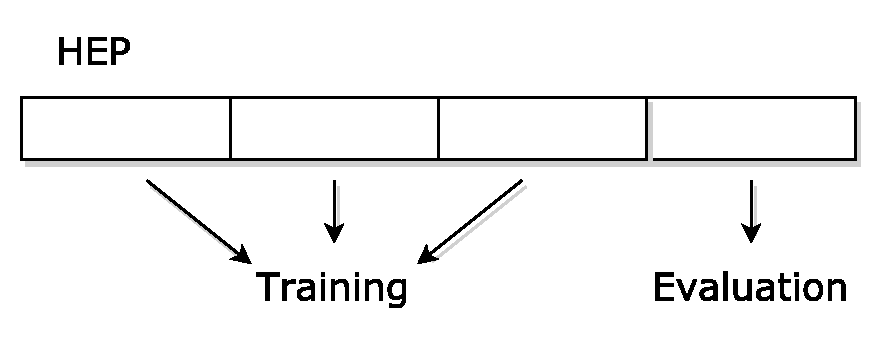
\includegraphics[width=0.36\textwidth]{Figures/CV_HEP.pdf}} & 
\subfloat[CV CORA]{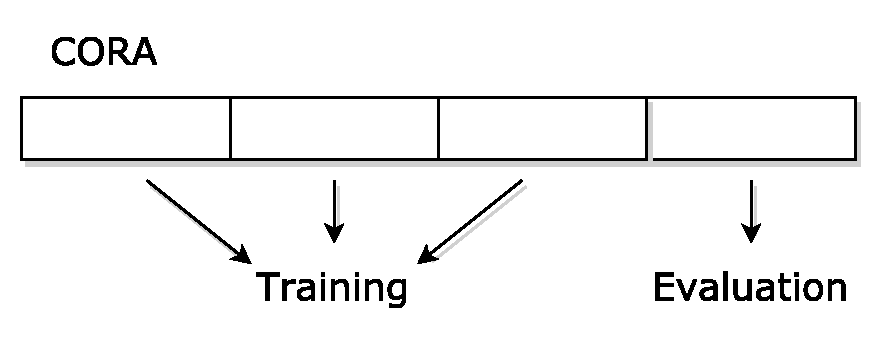
\includegraphics[width=0.36\textwidth]{Figures/CV_CORA.pdf}}\\
\subfloat[CV HEP append CORA]{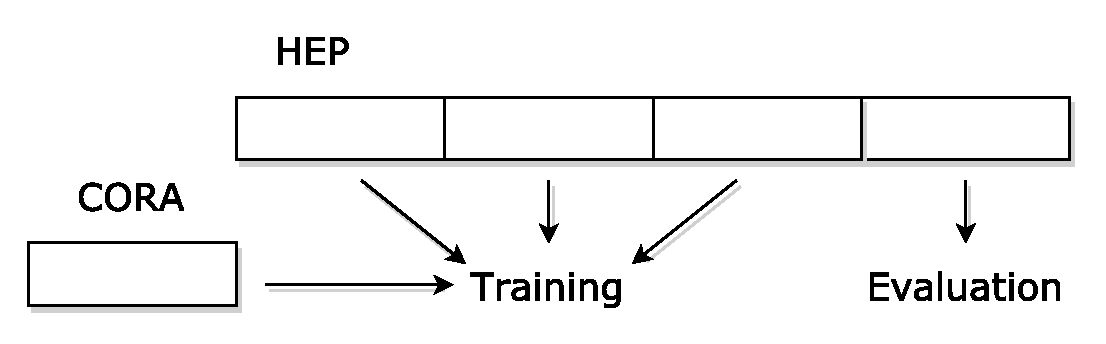
\includegraphics[width=0.45\textwidth]{Figures/CV_HEPappCORA.pdf}} & 
\subfloat[CV CORA append HEP]{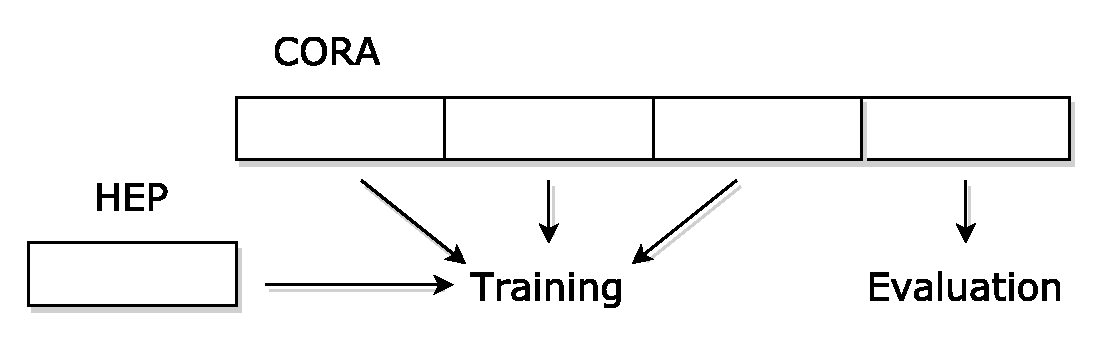
\includegraphics[width=0.45\textwidth]{Figures/CV_CORAappHEP.pdf}}\\ 
% \multicolumn{2}{c}{\subfloat[CV HEP + CORA]{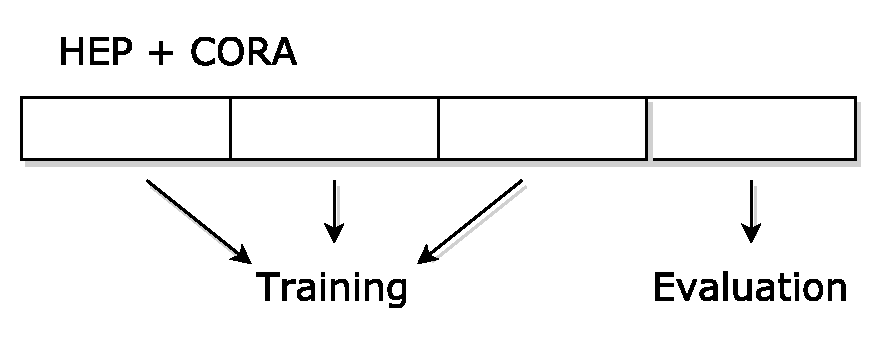
\includegraphics[width=0.36\textwidth]{Figures/CV_HEP+CORA.pdf}}} \\
\end{tabular}
\caption{The different cross-validation configurations used in our experiments. Figures (A) and (B) show cross-validation on HEP and CORA sets independently. Figures (C) and (D) show cross-validation on the HEP and CORA datasets respectively, appending the other at training time.}
\label{fig:cv}
\end{figure}

The variety of $66$ experiments that we cross-validated are presented in Table \ref{fig:cv}, organised into 8 categories. We also distinguish by model, running some experiments for both models, and some for one alone. Generally speaking, we chose feature engineering ideas with a particular model in mind, that is, either \emph{header} or \emph{segmentation}. Finally, we distinguish by data configuration. For dictionary-based features, which may be derived from a baseline feature file alone, we may try all data configurations. However, as we do not have access to the original PDF papers for the CORA dataset, we can only extract our other feature ideas on the HEP dataset.

\begin{table}[h]
\begin{center}
\begin{tabular}{ | p{0.2\linewidth} | p{0.25\linewidth} | p{0.15\linewidth} | p{0.3\linewidth} |}
\hline
Feature Category & Variations & Models & Data\\
\hline
\multirow{2}{*}{Baseline} & \multirow{2}{*}{-} & Segmentation, header & CORA, CORA app. HEP, CORA + HEP, HEP, HEP app. CORA \\
\cline{3-4}
 & & Header & HEP app. 1/3 CORA, HEP app. 2/3 CORA \\
\hline
Dictionaries & 1\textsuperscript{st} order, 2\textsuperscript{nd} order, 3\textsuperscript{rd} order & Segmentation, header & HEP, HEP app. CORA \\
\hline
Dicts. + Stops & 1\textsuperscript{st} order, 2\textsuperscript{nd} order, 3\textsuperscript{rd} order, stops only & Segmentation, header & HEP, HEP app. CORA \\
\hline
Regularisation & $\sigma^2=0$, $\sigma^2 = 10^{-6}$, $\sigma^2 = 10^{-5}$, $\sigma^2 = 10^{-4}$, $\sigma^2 = 10^{-3}$, & Header & HEP \\
\hline
Token Extension & First 5 words, first 10, first 15, first 20 & Segmentation & HEP \\
\hline
Block Size & Height, width, height \& width, area & Header & HEP \\
\hline
Levenshtein Distance & $T_1 = 0.05$, $T_1 = 0.1$, $T_1 = 0.2$, $T_1 = 0.4$, $T_1 = 0.8$, ($T_1 = 0.1, T_2 = 0.4$), All & Segmentation & HEP \\
\hline
Character Classes & Binary, decimal (round down), decimal (round), decimal (20 point) & Segmentation & HEP \\
\hline
\end{tabular}
\caption[A summary of our experiments, organised by category, models trained for, and data configurations used.]{A summary of our experiments, organised by category, models trained for, and data configurations used.}
\label{table:experiments}
\end{center}
\end{table}

\section{Comparison with \emph{refextract}}
\label{sec:refextract}

As a first result for GROBID, we compare its reference list classification performance with that of \emph{refextract}, the existing solution for automatic reference extraction at CERN. \emph{refextract} is an example of a \emph{stylistic analysis} tool (see Section \ref{sec:solutionmethods}), as it employs regular expressions in a heuristic framework for metadata extraction. As previously mentioned, \emph{refextract} is incomplete and greatly lacking in both breadth and depth of detail. It is capable only of retrieving an article's references\footnote{A comparatively easy task; GROBID's citation model usually performs at a significantly higher accuracy than, say, its \emph{header} model.}, and the classification itself is quite simplistic. Since the modelling of reference classes differs between the two, a comparison is difficult to make. Our results will however be at least indicative and we are able to make reasonable comparisons across the most important classes. The dataset for the comparison consists of 60 articles retrieved from the SCOAP$^3$ online repository\footnote{SCOAP$^3$ (Sponsoring Consortium for Open Access Publishing in Particle Physics) is an open access digital library hosted at CERN, backed by an international partnership of research institutions.}.

Unlike \emph{refextract}, GROBID requires two separate models to classify the citations of a given article: the \emph{reference-segmenter} and \emph{citation} models\footnote{Strictly speaking, there is another model, (full) \emph{segmentation}, above the \emph{reference-segmenter}, and so \emph{citation} accuracy depends on this also. But because one focus of our work is to improve this model, we permit this omission.}. The \emph{reference-segmenter} model is the simplest model in GROBID's arsenal, and is responsible for segmenting a reference list block into individual references. It does this by modelling two classes, <label>, the delimiting tokens between individual references, and <reference>. Therefore, the accuracy of the citation model is ultimately subject to the accuracy of the reference block inputs supplied it by the \emph{reference-segmenter} above. The results for training and evaluating the \emph{reference-segmenter} on 60 SCOAP$^3$ papers with an 80--20 split are given in Table \ref{table:referencesegmenterresults}. The results show the \emph{reference-segmenter} to be extremely accurate. In fact, only 5 token misclassifications out of 622 were made for the <label> class, and from a grand total of 12,981.

\begin{table}[h]
\begin{center}
\begin{tabular}{|c|cccc|}
\hline
label           & accuracy  & precision  & recall   & f1 \\
\hline
<label>         & 99.96     & 100        & 99.2     & 99.6\\
<reference>     & 99.96     & 99.96      & 100      & 99.98\\
\hline
(micro average) & 99.96     & 99.96      & 99.96    & 99.96  \\
(macro average) & 99.96     & 99.98      & 99.6     & 99.79  \\
\hline
\end{tabular}
\caption[Token-level evaluation results for reference segmentation.]{Token-level evaluation results for reference segmentation.}
\label{table:referencesegmenterresults}
\end{center}
\end{table}

The most significant difference between the tools is the set of classes modelled. \emph{refextract} attempts only to classify to the minimum detail required for identifying the originating document within INSPIRE-HEP. Therefore, there are no equivalents to GROBID's classes, <volume>, <pages>, and so on. Rather, these parts of references are absorbed into other, higher-level classes, and are indicated by a dash (-) in the results table, Table \ref{table:citationcomparison}. Comparisons can be made, however, on fields, <title>, <author>, <journal>, and <date>. There we see the superiority of GROBID over \emph{refextract}. Note that here the \emph{citation} model was not trained on the evaluation set, and in particular this may explain its dismal performance in precision for the <date> class, and recall for <pubnum>. The dataset instances contained a recurring publication number that was almost uniformly misclassified by GROBID as a date. Notice that this is an example of a domain specificity of HEP papers. Had we trained on these papers, we could expect an improvement. That \emph{refextract} has reported perfect recall is the result of a flaw in our simplistic evaluation, where missing expected classifications were simply assigned to a <null> class, and so \emph{false positives} (FP) were not counted; only \emph{false negatives} (FN). Therefore, the true performance of \emph{refextract} is upper-bounded by the figures in Table \ref{table:citationcomparison}. The table contents are one of the outputs of GROBID's evaluation utilities. For an explanation of the performance metrics, see Section \ref{subsec:evaluationmethod}.

\begin{table}[h]
\begin{center}
\begin{tabular}{|c|cccc|cccc|}
\hline
system &  \multicolumn{4}{c|}{GROBID} & \multicolumn{4}{c|}{\emph{refextract}}\\
\hline
label & accuracy & precision & recall & f1 & acc. & prec. & rec. & f1\\
\hline
<author>    & 99.85 &   99.68   &   99.75   &   99.72   & 98.33 &   100 &   92.22   &   95.95   \\
<title> &   99.59   &   98.87   &   99.25   &   99.06   & 94.89 &   100 &   71.75   &   83.55   \\
<journal>   & 98.84 &   88.87   &   93.98   &   91.35   & 97.12 &   100 &   46.78   &   63.74   \\
<volume>&   99.95   &   99.07   &   98.15   &   98.6    & -     &   -   &   -       &   -   \\
<issue> &   99.93   &   100     &   94.63   &   97.24   & -     &   -   &   -       &   -   \\
<pages> &   99.75   &   93.51   &   99.45   &   96.39   & -     &   -   &   -       &   -   \\
<date>  &   98.39   &   57.39   &   98.31   &   72.47   & 98.88 &   100 &   37.55   &   54.6    \\
<pubnum>&   98.71   &   100     &   12.96   &   22.95   & -     &   -   &   -       &   -   \\
<note>  &   99.4    &   43.75   &   35      &   38.89   & -     &   -   &   -       &   -   \\
<publisher>&99.81   &   63.46   &   94.29   &   75.86   & -     &   -   &   -       &   -   \\
<location>& 99.81   &   86.32   &   91.11   &   88.65   & -     &   -   &   -       &   -   \\
<institution>& 99.78&   25      &   25      &   25      & -     &   -   &   -       &   -   \\
<booktitle>&    98.7&   55.56   &   41.67   &   47.62   & -     &   -   &   -       &   -   \\
<web>   &   99.64   &   51.85   &   100     &   68.29   & -     &   -   &   -       &   -   \\
<editor>    &  99.93&   100     &	46.67   &   63.64   & -     &   -   &   -       &   -   \\
<tech>  &   99.95   &   83.33   &   50      &   62.5    & -     &   -   &   -       &   -   \\
\hline
(micro average) & 99.5  &   93.63   &   94.77   &   94.19 & -    &   - &   -   &   -   \\
(macro average) & 99.5  &   77.92   &   73.76   &   71.76 & -    &   -  &   -   &   -   \\
\hline
\end{tabular}
\caption[Token-level evaluation results of citation extraction for GROBID and \emph{refextract}.]{Token-level evaluation results for citations for GROBID and \emph{refextract}.}
\label{table:citationcomparison}
\end{center}
\end{table}

\section{Results}
\label{sec:results}

As specified earlier, we use the micro average of $F_1$ scores of all model classes to compare model performance, only looking to specific fields when more nuanced comparisons are required. We hereafter state $F_1$ micro averages unless otherwise specified. Note that Section \ref{sec:keyresults} presents the key results and comparisons from this section.

\subsection{Baseline}
\label{subsec:baslineresults}

Given the datasets available (see Section \ref{sec:data}), we are able to experiment with combinations of HEP and CORA papers, as well as with subsampling the CORA dataset to find the ideal mixture. After all, in spite of the common wisdom that increasing the amount of training data will improve generalisation and model performance, it is not clear what effects combining different ground truths will have. One may imagine that generalising over a hybrid dataset might learn a model that is misleading when it comes to evaluate on a pure HEP dataset, especially when the CORA \emph{header} set dwarfs our HEP one. The baseline results are given in Table \ref{table:baselineresults} and these show the micro average of $F_1$ scores (see Section \ref{subsec:evaluationmethod}) for each of the data configurations. Of most importance are the scenarios involving the HEP training set taken alone, and the HEP training set appending the CORA set, as these evaluate on HEP papers only, and are the configurations used in the other experiments. Surprisingly, for the \emph{header} model, there is a degradation of performance when the CORA set is appended. We pursue this curiosity in Table \ref{table:subsampling}, where we see mixed results for \emph{subsampling} CORA data, appending an extra, randomly chosen third of the $2506$ training instances each time. The pure HEP set with no appending of CORA data $(\mu = 90.19, \sigma = 2.63)$ yields a model second only to the case where we append $2/3$ of the CORA dataset $(\mu = 92.1, \sigma = 2.43)$. The case of appending $1/3$ CORA experienced a major outlier in the third iteration of cross-validation, where it scored an $F_1$ micro average of as little as $78.15$, performing badly across all classes. This result notwithstanding, it seems there is some value in using a hybrid dataset, yet increasing the proportion of CORA papers ultimately degrades performance. This strongly supports our hypothesis that there a qualitative difference between HEP papers and general papers, but that training a successful model demands an expansion of the HEP dataset. In further sections, we see the same effect when we train on the HEP dataset and HEP appending CORA. For a visualisation of the subsampling results, see Figure \ref{fig:subsampling_micro} in Appendix \ref{AppendixB}. The successful predictions of our newly introduced collaboration class for the header model (see Section \ref{subsec:extensions}) should be noted also.

\begin{table}[t]
\begin{center}
\begin{tabular}{|c|c|c|c|c|}
\hline
Model & Variation & Data & Mean & Std.\\
\hline
\multirow{4}{*}{Header} & \multirow{4}{*}{-} & HEP & 90.19 & 2.63\\\cline{3-5}
& & HEP app. CORA & 89.54 & 3.76\\\cline{3-5}
& & CORA & 82.22 & 2.03\\\cline{3-5}
& & CORA app. HEP & 81.8 & 2.76\\\cline{3-5}
\hline
\multirow{4}{*}{Segmentation} & \multirow{4}{*}{-} & HEP & 92.98 & 0.79\\\cline{3-5}
& & HEP app. CORA & 93.58 & 1.65\\\cline{3-5}
& & CORA & 94.02 & 2.96\\\cline{3-5}
& & CORA app. HEP & 94.39 & 2.72\\\cline{3-5}
\hline
\end{tabular}
\caption{Mean and standard deviation for baseline data configurations.}
\label{table:baselineresults}
\end{center}
\end{table}

\begin{table}[t]
\begin{center}
\begin{tabular}{|c|c|c|c|c|}
\hline
Model & Variation & Data & Mean & Std.\\
\hline
\multirow{4}{*}{Header} & \multirow{4}{*}{-} & HEP & 90.19 & 2.63\\\cline{3-5}
& & HEP app. 1/3 CORA & 89.15 & 5.75\\\cline{3-5}
& & \textbf{HEP app. 2/3 CORA} & \textbf{92.1} & \textbf{2.43}\\\cline{3-5}
& & HEP app. CORA & 89.54 & 3.76\\\cline{3-5}
\hline
\end{tabular}
\caption{Mean and standard deviation for subsampling CORA dataset.}
\label{table:subsampling}
\end{center}
\end{table}

In contrast, the \emph{segmentation} model generally benefited from combining datasets, with HEP appending CORA $(\mu = 93.58, \sigma = 1.65)$ and CORA appending HEP $(\mu = 94.39, \sigma = 2.72)$ respectively improving over HEP alone $(\mu = 92.98, \sigma = 0.79)$ and CORA alone $(\mu = 94.02, \sigma = 2.96)$. This seems reasonable, as the HEP set in this case is larger than the CORA one, and appending the CORA dataset can assist model performance without overwhelming the HEP characteristics as it does for the \emph{header} model. Figure \ref{fig:segmentation_baseline_confusion} gives a confusion matrix for the \emph{segmentation} model evaluated with the baseline features on the HEP training set. The main diagonal (in dark blue) shows the majority correctness of the model. Notably, the <body> class (the lines belonging to the main article sections) shows a high true positive (TP) rate (observe the contrast in the <body> row), but also a high number of false positives (observe the confusion in the <body> column), equivalently, the false \emph{negatives} of other classes. Thus, lower precision and higher recall. This is to be expected, as <body> is the dominant class for the \emph{segmentation} model, and training error is most easily minimised with a bias to the dominant class (a similar result may be seen in Figure \ref{fig:confusion_header} in Appendix \ref{AppendixB} for the <abstract> class in the \emph{header} model). The confusion matrix also reveals large amounts of header matter lost to the <body> class. This is of greatest concern, as the extracted data ought to supply the \emph{header} model with its inputs at prediction time. One of our extensions to GROBID (Section \ref{subsec:extensions}) allows us to see which documents these misclassifications are most attributed to.

\begin{figure}[h]
\center
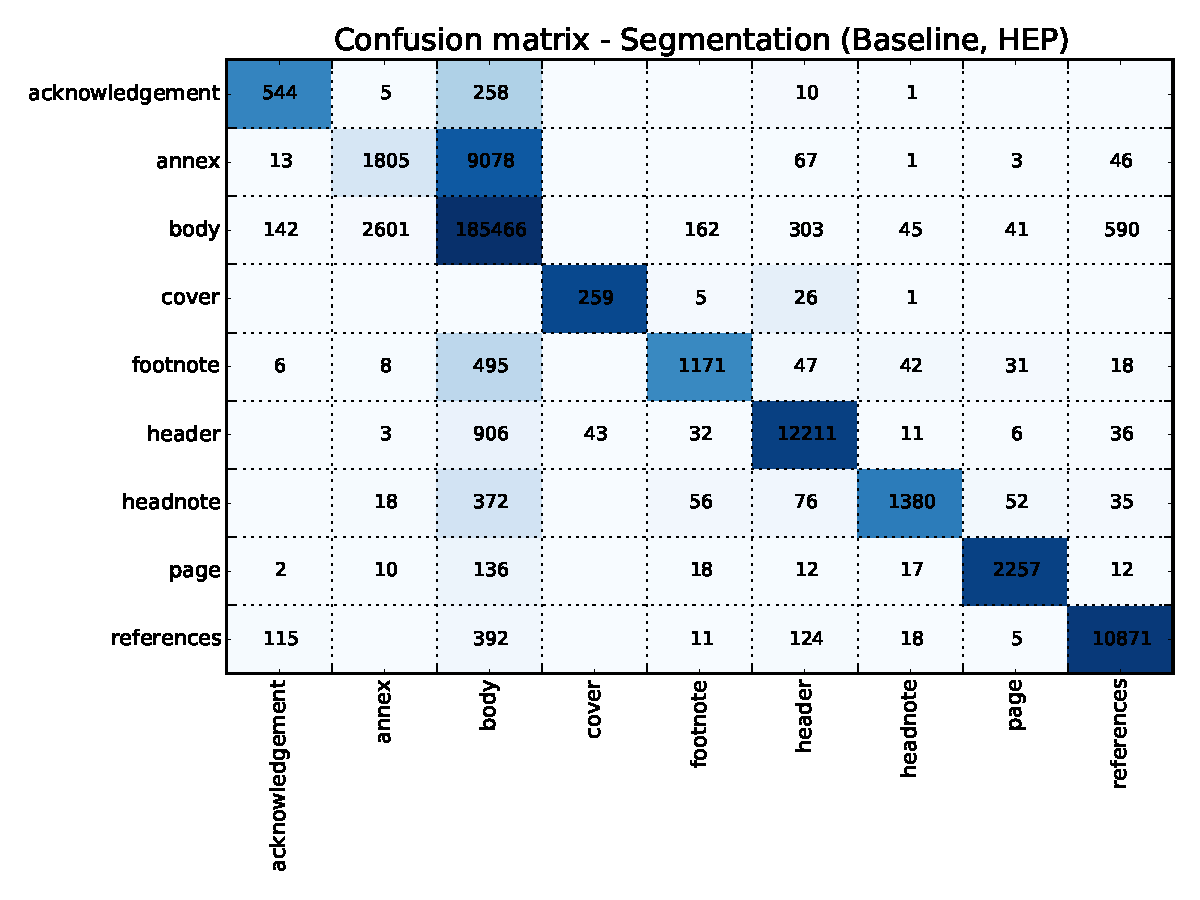
\includegraphics[width=5.5in]{Figures/baseline_confusion_segmentation.pdf}
\caption{Confusion matrix for \emph{segmentation} model with baseline features, trained on the pure HEP dataset. Counts are given, as well as a heatmap to indicate the most frequent classifications.}
\label{fig:segmentation_baseline_confusion}
\end{figure}

\subsection{Block Size}

\begin{table}[h]
\begin{center}
\begin{tabular}{|c|c|c|c|c|}
\hline
Model & Variation & Data & Mean & Std.\\
\hline
\multirow{5}{*}{Header} & \emph{Baseline} & \emph{HEP} & \emph{90.19} & \emph{2.63} \\\cline{2-5}
& \textbf{Height} & \textbf{HEP} & \textbf{90.5} & \textbf{2.55}\\\cline{2-5}
& Width & HEP & 90.46 & 2.75\\\cline{2-5}
& Height \& width & HEP  & 88.47 & 3.1\\\cline{2-5}
& Area & HEP  & 90.42 & 2.55\\\cline{2-5}
\hline
\end{tabular}
\caption{Mean and standard deviation for block size variations.}
\label{table:blockshaperesults}
\end{center}
\end{table}

The results for our block size features (Table \ref{table:blockshaperesults}) were not significant, with only the most marginal differences with respect to the baseline $(\mu = 90.19, \sigma = 2.63)$. The category using both height and width features performed worst $(\mu = 88.47, \sigma = 3.1)$, showing that combining features does not necessarily improve, and may even degrade, model performance, a finding we see elsewhere also\footnote{Notably the combination of our best features for \emph{segmentation}. Future work might examine the correlation of independent features to see if a methodology for combining features may be derived.}. The results are otherwise quite uniform. We may speculate as to the underwhelming performance of these features by noticing that block size is calculated for every token according to its membership in a contiguous group of tokens. As a result, contiguous tokens share identical information on block sizes, and these features do nothing to \emph{characterise} the tokens individually in the way successful features such as \emph{character classes} (Section \ref{subsec:characterclassresults}) and  \emph{dictionaries} (Section \ref{subsec:dictionaries}) do.

\subsection{Character Classes}
\label{subsec:characterclassresults}

Almost every character class strategy made an improvement over the baseline (with the exception of the simple \emph{binary} variation). A visualisation of the results may be seen in Figure \ref{fig:classes_micro} in Appendix \ref{AppendixB}. Thus, the results support our intuitions about features based on character classes. The variations \emph{binary only} and \emph{decimal only} refer to the removal of the basic baseline features addressing punctuation and related line token characteristics. Interestingly, removing these baseline features \emph{improved} performance, even for the baseline feature set alone. The best micro average result was for the \emph{20-point} variation $(\mu = 93.75, \sigma = 2.56)$ compared with the baseline, $(\mu = 92.98, \sigma = 0.79)$, corresponding to an $11\%$ reduction in error on the micro average level, as well as a $20\%$ reduction in error ($F_1$) for <header>, and a $13\%$ reduction in error for <references>, the two most important classes. The \emph{20-point} variation used a finer discretisation than the others. Future work might therefore try further refining the discretisation strategies. However, the runner-up, \emph{decimal only} $(\mu = 93.69, \sigma = 1.99)$, gave a $24\%$ reduction for the <header> class, and $21\%$ for <references>. We therefore favour this variation, and short-list it for our further comparisons (see Section \ref{sec:keyresults}).

\begin{table}[h]
\begin{center}
\begin{tabular}{|c|c|c|c|c|}
\hline
Model & Variation & Data & Mean & Std.\\
\hline
\multirow{7}{*}{Segmentation} & \emph{Baseline} & \emph{HEP} & \emph{92.98} & \emph{0.79} \\\cline{2-5}
& Binary & HEP & 92.82 & 1.26\\\cline{2-5}
& Binary only & HEP & 93.5 & 2.17\\\cline{2-5}
& Decimal (round down) & HEP & 93.57 & 2.2\\\cline{2-5}
& Decimal only & HEP & 93.61 & 1.99\\\cline{2-5}
& Decimal (round nearest) & HEP & 93.37 & 2.27\\\cline{2-5}
& \textbf{Decimal (20 point)} & \textbf{HEP} & \textbf{93.75} & \textbf{2.56}\\\cline{2-5}
\hline
\end{tabular}
\caption{Mean and standard deviation for character class discretisation strategies.}
\label{table:characterclassresults}
\end{center}
\end{table}

\subsection{Dictionaries}
\label{subsec:dictionaries}
Dictionary-based features, as described in Section \ref{subsec:dicts}, make use of domain knowledge to establish a vocabulary for \emph{header} model tokens and give a binary indicator, modelling a token's memberships in a set of five dictionaries (titles, authors, journals, collaborations, and keywords), extracted from INSPIRE-HEP. We varied the degree of context-awareness provided to a token, creating features indicating the dictionary membership of a token's immediate neighbours, that is, the tokens either side of it in the text, in addition to its own membership, as well as second and third degree neighbours. The results for these variations are given in Table \ref{table:dictionaryresults}. Though these features were designed with the \emph{header} model in mind, the same experimental variations were run for \emph{segmentation}. The features were expected to be more meaningful for the \emph{header} model, as they give a dimensionality reduction for a full token, mapping it to some combination of dictionaries. In the \emph{segmentation} model, this is done only for the leading word per line, and it is hard to imagine this characterising a line effectively. Predictably, the \emph{header} model benefited significantly more from dictionary-based features, with clear improvements over the baseline: $(\mu =  90.19, \sigma = 2.63)$ for the \emph{header} model trained on HEP, and $(\mu =  92.98, \sigma = 0.79)$ for the \emph{segmentation} model. The most successful variation was the 1\textsuperscript{st} degree for both \emph{header} $(\mu = 90.75, \sigma = 2.5)$ and \emph{segmentation} $(\mu = 93.91, \sigma = 2.07)$ models. When stop words were included (Table \ref{table:dictsstopsresults}) the benefits were even greater for the \emph{header} model. This reflects the significant varying of stop word frequency between classes discovered in Section \ref{sec:stopwordfrequency} in Appendix \ref{AppendixC}. The most successful variation in this case was the 3\textsuperscript{rd} degree for both \emph{header} $(\mu = 91.35, \sigma = 3.1)$ and \emph{segmentation} $(\mu = 93.58, \sigma = 2.66)$ models. The results for the \emph{header} models are selected for closer examination in Section \ref{sec:keyresults}. Of further note was the near uniform superiority of the pure HEP data configuration versus that of appending CORA data, reinforcing our findings about subsampling from the baseline results (Section \ref{subsec:baslineresults}. It is after this experiment batch that we choose to be more focused in the scenarios chosen, concentrating on the pure HEP dataset and the models expected to most benefit from the respective feature experiments.

\begin{table}[h]
\begin{center}
\begin{tabular}{|c|c|c|c|c|}
\hline
Model & Variation & Data & Mean & Std.\\
\hline
\multirow{7}{*}{Header} & \emph{Baseline} & \emph{HEP} & \emph{90.19} & \emph{2.63} \\\cline{3-5}
& \multirow{2}{*}{\textbf{1\textsuperscript{st} order}} & \textbf{HEP} & \textbf{90.75} & \textbf{2.5}\\\cline{3-5}
& & HEP app. CORA & 87.65 & 6.49\\\cline{2-5}
& \multirow{2}{*}{2\textsuperscript{nd} order} & HEP & 90.75 & 3.01\\\cline{3-5}
& & HEP app. CORA & 88.78 & 7.46\\\cline{2-5}
& \multirow{2}{*}{3\textsuperscript{rd} order} & HEP & 87.67 & 7.55\\\cline{3-5}
& & HEP app. CORA & 89.78 & 5.99\\ \hline
\multirow{7}{*}{Segmentation} & \emph{Baseline} & \emph{HEP} & \emph{92.98} & \emph{0.79} \\\cline{2-5}
& \multirow{2}{*}{\textbf{1\textsuperscript{st} order}} & HEP & 93.56 & 1.79\\\cline{3-5}
& & \textbf{HEP app. CORA} & \textbf{93.91} & \textbf{2.07}\\\cline{2-5}
& \multirow{2}{*}{2\textsuperscript{nd} order} & HEP & 92.16 & 1.61\\\cline{3-5}
& & HEP app. CORA & 93.37 & 1.75\\\cline{2-5}
& \multirow{2}{*}{3\textsuperscript{rd} order} & HEP & 93.11 & 2.6\\\cline{3-5}
& & HEP app. CORA & 93.58 & 1.89\\
\hline
\end{tabular}
\caption{Mean and standard deviation for dictionary features.}
\label{table:dictionaryresults}
\end{center}
\end{table}

\begin{table}[h]
\begin{center}
\begin{tabular}{|c|c|c|c|c|}
\hline
Model & Variation & Data & Mean & Std.\\
\hline
\multirow{7}{*}{Header} & \emph{Baseline} & \emph{HEP} & \emph{90.19} & \emph{2.63} \\\cline{2-5}
& \multirow{2}{*}{1\textsuperscript{st} order} & HEP & 91.21 & 2.03\\\cline{3-5}
& & HEP app. CORA & 88.43 & 5.92\\\cline{2-5}
& \multirow{2}{*}{2\textsuperscript{nd} order} & HEP & 88.9 & 7.25\\\cline{3-5}
& & HEP app. CORA & 89.87 & 5.03\\\cline{2-5}
& \multirow{2}{*}{\textbf{3\textsuperscript{rd} order}} & \textbf{HEP} & \textbf{91.35} & \textbf{3.1}\\\cline{3-5}
& & HEP app. CORA & 89.76 & 5.99\\ \hline
\multirow{7}{*}{Segmentation} & \emph{Baseline} & \emph{HEP} & \emph{92.98} & \emph{0.79} \\\cline{2-5}
& \multirow{2}{*}{1\textsuperscript{st} order} & HEP & 93.21 & 1.13\\\cline{3-5}
& & HEP app. CORA & 93.48 & 2.04\\\cline{2-5}
& \multirow{2}{*}{2\textsuperscript{nd} order} & HEP & 93.03 & 1.78\\\cline{3-5}
& & HEP app. CORA & 93.24 & 3.49\\\cline{2-5}
& \multirow{2}{*}{\textbf{3\textsuperscript{rd} order}} & HEP & 93.25 & 2.77\\\cline{3-5}
& & \textbf{HEP app. CORA} & \textbf{93.58} & \textbf{2.66}\\
\hline
\end{tabular}
\caption{Mean and standard deviation for dictionary features combined with stop word features.}
\label{table:dictsstopsresults}
\end{center}
\end{table}

\subsection{Levenshtein Distance}

All Levenshtein distance feature thresholding strategies performed better than the baseline, and the scenarios combining multiple thresholds, ($T_1 = 0.1, T_2 = 0.4$) and \emph{All}, show a clear superiority over the others. A visualisation of the results can be seen in Figure \ref{fig:levenshtein_micro} in Appendix \ref{AppendixB}. The strategy, \emph{All}, which used all of the listed thresholds to make a $5-point$ categorical variable based on Levenshtein distance gave the best performance, $(\mu = 94.06, \sigma = 1.81)$, compared with the baseline, $(\mu = 92.98, \sigma = 0.79)$, corresponding to a $15\%$ reduction in error on the micro average level, as well as a $20\%$ reduction in error for <references>, and a $19\%$ reduction in error for the <header>. These results therefore support our intuitions of the effectiveness of this feature category. Such as it is, from the laborious data acquisition process (Section \ref{sec:data}), we observed the frequency of the misclassification of delimiting token classes, <page> and <headnote>, as part of the <body> or <reference> sections, raising the false positive (FP) rate for these classes, thus lowering their precision and $F_1$ scores alike. It is therefore likely that the Levenshtein distance features aided these transitional corner cases in the document segmentation. The most successful Levenshtein distance variety is compared in more detail in Section \ref{sec:keyresults}. 

\begin{table}[h]
\begin{center}
\begin{tabular}{|c|c|c|c|c|}
\hline
Model & Variation & Data & Mean & Std.\\
\hline
\multirow{7}{*}{Segmentation} & \emph{Baseline} & \emph{HEP} & \emph{92.98} & \emph{0.79} \\\cline{2-5}
& $T_1 = 0.1$ & HEP & 93.51 & 1.37\\\cline{2-5}
& $T_1 = 0.2$ & HEP & 92.95 & 1.19\\\cline{2-5}
& $T_1 = 0.4$ & HEP & 93.44 & 1.28\\\cline{2-5}
& $T_1 = 0.8$ & HEP & 93.07 & 1.07\\\cline{2-5}
& $T_1 = 0.1, T_2 = 0.4$ & HEP & 93.78 & 1.83\\\cline{2-5}
& \textbf{All} & \textbf{HEP} & \textbf{94.06} & \textbf{1.81}\\\cline{2-5}
\hline
\end{tabular}
\caption{Mean and standard deviation for Levenshtein distance thresholding variations.}
\label{table:levenshteinresults}
\end{center}
\end{table}

\subsection{Regularisation}

\begin{figure}[h]
\center
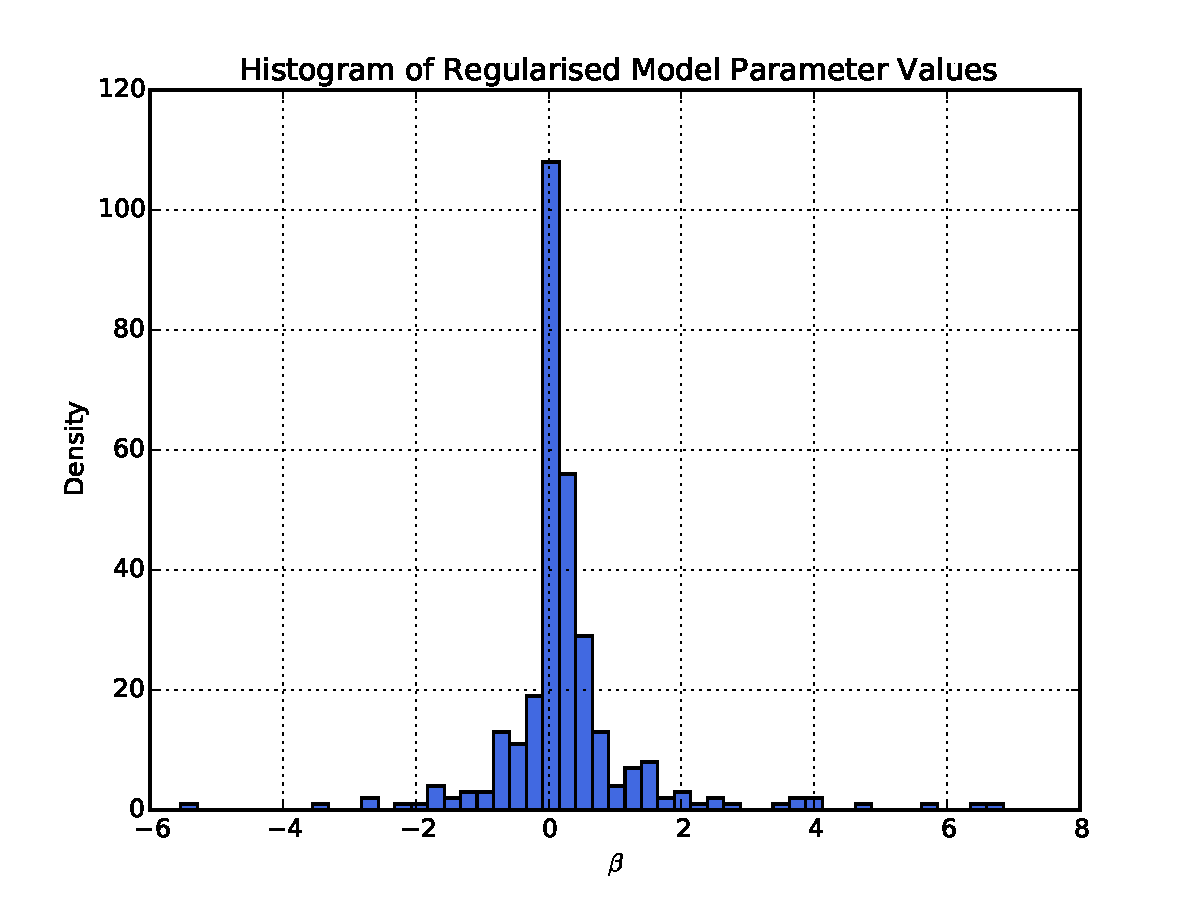
\includegraphics[width=5.5in]{Figures/histogram.pdf}
\caption{Distribution of model parameters with $l_2$ regularisation.}
\label{fig:histogram}
\end{figure}

Our experiments in tuning the variance of the $l_2$ regularisation confirmed the earlier findings of (\cite{Peng04accurateinformation}). There is little observable difference in the performance of different choices of variance parameter, which we give in Table \ref{table:regularisationresults}. Performance is marginally worse at the extremities, namely where no penalty is imposed, and for the greatest penalty, $\sigma^2 = 10^{-3}$. Naturally, as a penalty is increased toward infinity, the model parameters go to 0, and performance degrades maximally. Figure \ref{fig:histogram} shows an empirical Normal distribution for a normalised model. That regularisation has little effect implies that it is difficult to overfit the model, and that the high dimensionality of the model perhaps provides in-built regularisation. Training with another algorithm supporting a different regularisation technique (such as $l_1$) could form the basis of future work.

\begin{table}[h]
\begin{center}
\begin{tabular}{|c|c|c|c|c|}
\hline
Model & Variation & Data & Mean & Std.\\
\hline
\multirow{5}{*}{Header} & \emph{Baseline} & \emph{HEP} & \emph{90.19} & \emph{2.63} \\\cline{2-5}
& $\sigma^2 = 0$ & HEP & 90.4 & 2.58\\\cline{2-5}
& $\mathbf \sigma^2 = 10^{-6}$ & HEP & 90.68 & 3.78\\\cline{2-5}
& $\sigma^2 = 10^{-5}$ & HEP & 90.64 & 3.78\\\cline{2-5}
& $\sigma^2 = 10^{-4}$ & HEP & 90.66 & 3.69\\\cline{2-5}
& $\sigma^2 = 10^{-3}$ & HEP & 90.44 & 2.77\\\cline{2-5}
\hline
\end{tabular}
\caption{Mean and standard deviation for tuning the variance of the $l_2$ variance parameter.}
\label{table:regularisationresults}
\end{center}
\end{table}

\subsection{Token Extensions}
\label{subsec:tokenextensionresults}

The results for token extensions (Table \ref{table:tokenextensions}) are quite modest. No variation significantly exceeds the baseline result with the same data configuration $(\mu = 92.98, \sigma = 0.79)$. Of note is the low variance across the variations compared with other feature categories. The result supports our earlier intuitions that though it may be helpful to establish a vocabulary that can differentiate between sections, the result of modelling each word in a line token individually is a feature space that is too diffuse to learn useful indicators, given that encountering the same combination of words occurs only rarely. Line tokens are therefore better characterised, for example, at the character- rather than word-level, such as by character class features (Section \ref{subsec:characterclassresults}).

\begin{table}[h]
\begin{center}
\begin{tabular}{|c|c|c|c|c|}
\hline
Model & Variation & Data & Mean & Std.\\
\hline
\multirow{5}{*}{Segmentation} & \emph{Baseline} & \emph{HEP} & \emph{92.98} & \emph{0.79} \\\cline{2-5}
& \textbf{First 5} & \textbf{HEP} & \textbf{93.38} & \textbf{1.6}\\\cline{2-5}
& First 10 & HEP & 92.8 & 1.08\\\cline{2-5}
& First 15 & HEP & 93.12 & 1.5\\\cline{2-5}
& First 20 & HEP & 93.29 & 1.75\\\cline{2-5}
\hline
\end{tabular}
\caption{Mean and standard deviation for token extension variations.}
\label{table:tokenextensions}
\end{center}
\end{table}

\section{Key Results}
\label{sec:keyresults}

In this section we visualise and discuss the most interesting and significant comparisons drawn from the results in Section \ref{sec:results}. We consider each model in turn, beginning with the \emph{header} model.

\subsection{Header Model}

The complexity of the \emph{header} model, modelling 17 classes (including our new <collaboration> class), made finding improvements difficult. Nevertheless, the model benefited from the five binary dictionary-based features, and further benefited from the additional stop word feature, functioning as a $6th$ dictionary. A comparison with the baseline on the HEP dataset is visualised in Figure \ref{fig:micro_header}, showing the micro average $F_1$ scores for each model. Dictionaries alone $(\mu = 90.75, \sigma = 2.5)$ reduced error over baseline $(\mu = 90.19, \sigma = 2.63)$ by $6\%$, and dictionaries with stop words $\pm 3$ (that is, third degree contextual awareness), by $12\%$. The latter, our best result for the \emph{header} model, corresponds with a $16\%$ error reduction for <address>, $19\%$ for <author>, $54\%$ for <collaboration>, $14\%$ for <date>, and $25\%$ for <keywords>, unchanged performance for <abstract>, <affiliation>, and <title>, and a slight degradation of $8\%$ for <pubnum>.

\begin{figure}[h]
\center
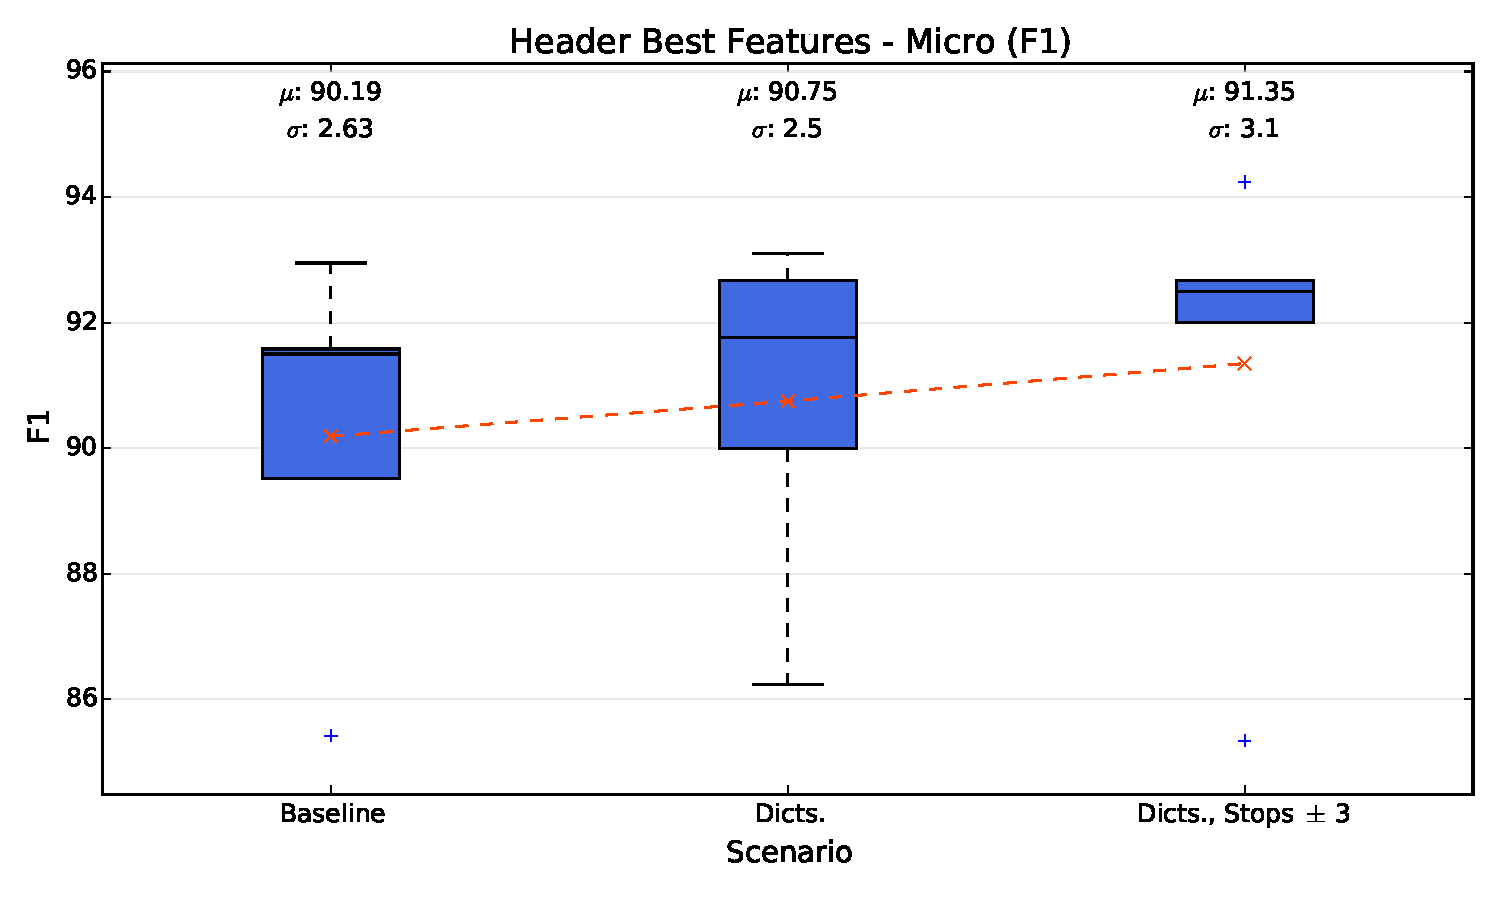
\includegraphics[width=5.5in]{Figures/micro_header.pdf}
\caption{Comparison of baseline, dictionary, and stop word features for overall \emph{header} model performance.}
\label{fig:micro_header}
\end{figure}

\subsection{Segmentation Model}

\begin{figure}[h]
\center
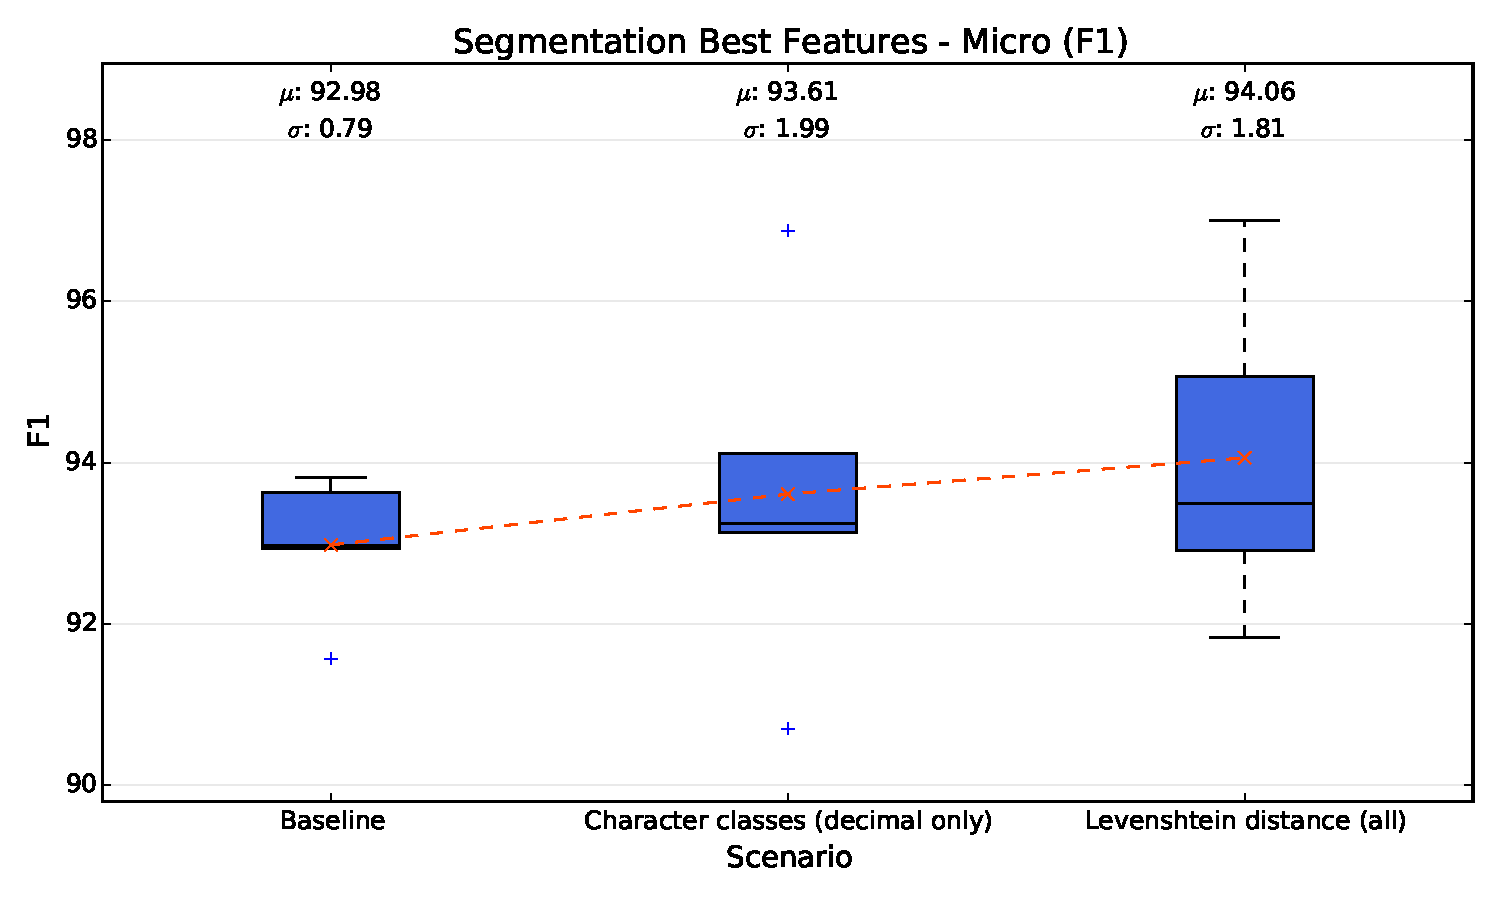
\includegraphics[width=5.5in]{Figures/micro_segmentation.pdf}
\caption{Comparison of baseline, Levenshtein distance and character class features for overall \emph{segmentation} model performance.}
\label{fig:micro_segmentation}
\end{figure}

For the \emph{segmentation} model, two feature categories offered significant improvements over the baseline. These categories were those of character classes (CC) and Levenshtein distance (LD), and their best variations were respectively the decimal discretisation with related baseline features removed (decimal only), and the Levenshtein distance feature using all thresholds to create a quinternary categorical variable. Figure \ref{fig:micro_segmentation} shows a boxplot comparing the micro average of $F_1$ scores of these two variations with the baseline, evaluated on the pure HEP dataset. The CC variation gives an overall error reduction of $9\%$, and the LD, $15\%$. However, when we look at the most important fields, <header> (Figure \ref{fig:header}) and <references> (Figure \ref{fig:references}), we see that though again both models outperform the baseline, now CC leads with a $24\%$ error reduction for the <header> class, with $19\%$ for LD, and a $21\%$ error reduction for <references> versus $20\%$ for LD. The character class model is therefore excelling in the cases it was explicitly designed to improve.

\begin{figure}[t]
\center
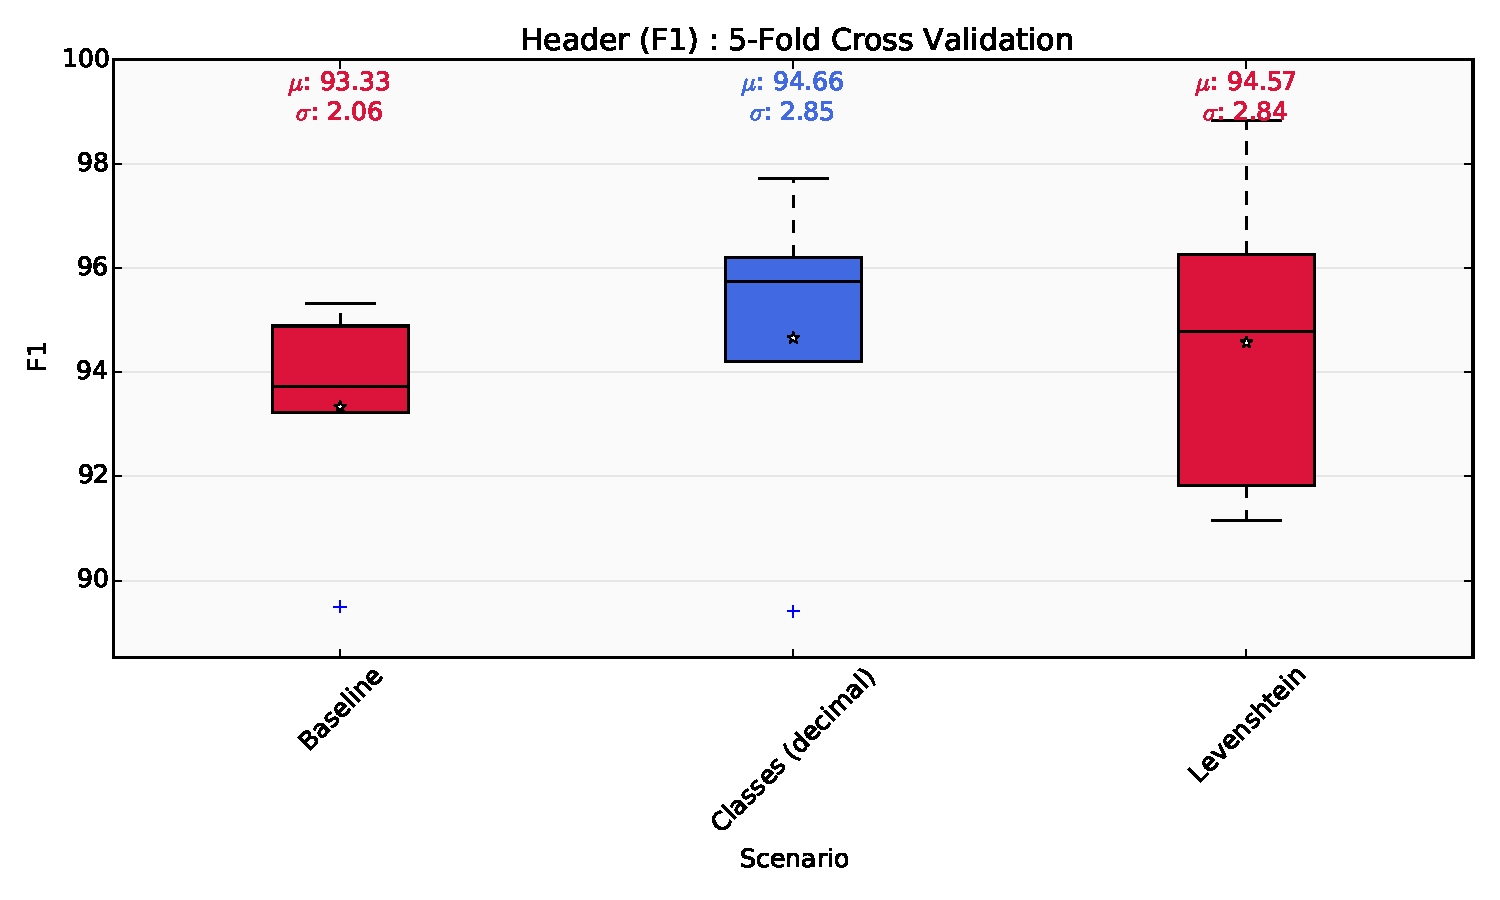
\includegraphics[width=5.5in]{Figures/header.pdf}
\caption{Comparison of baseline, Levenshtein distance and character class features for the header extraction.}
\label{fig:header}
\end{figure}

\begin{figure}[b]
\center
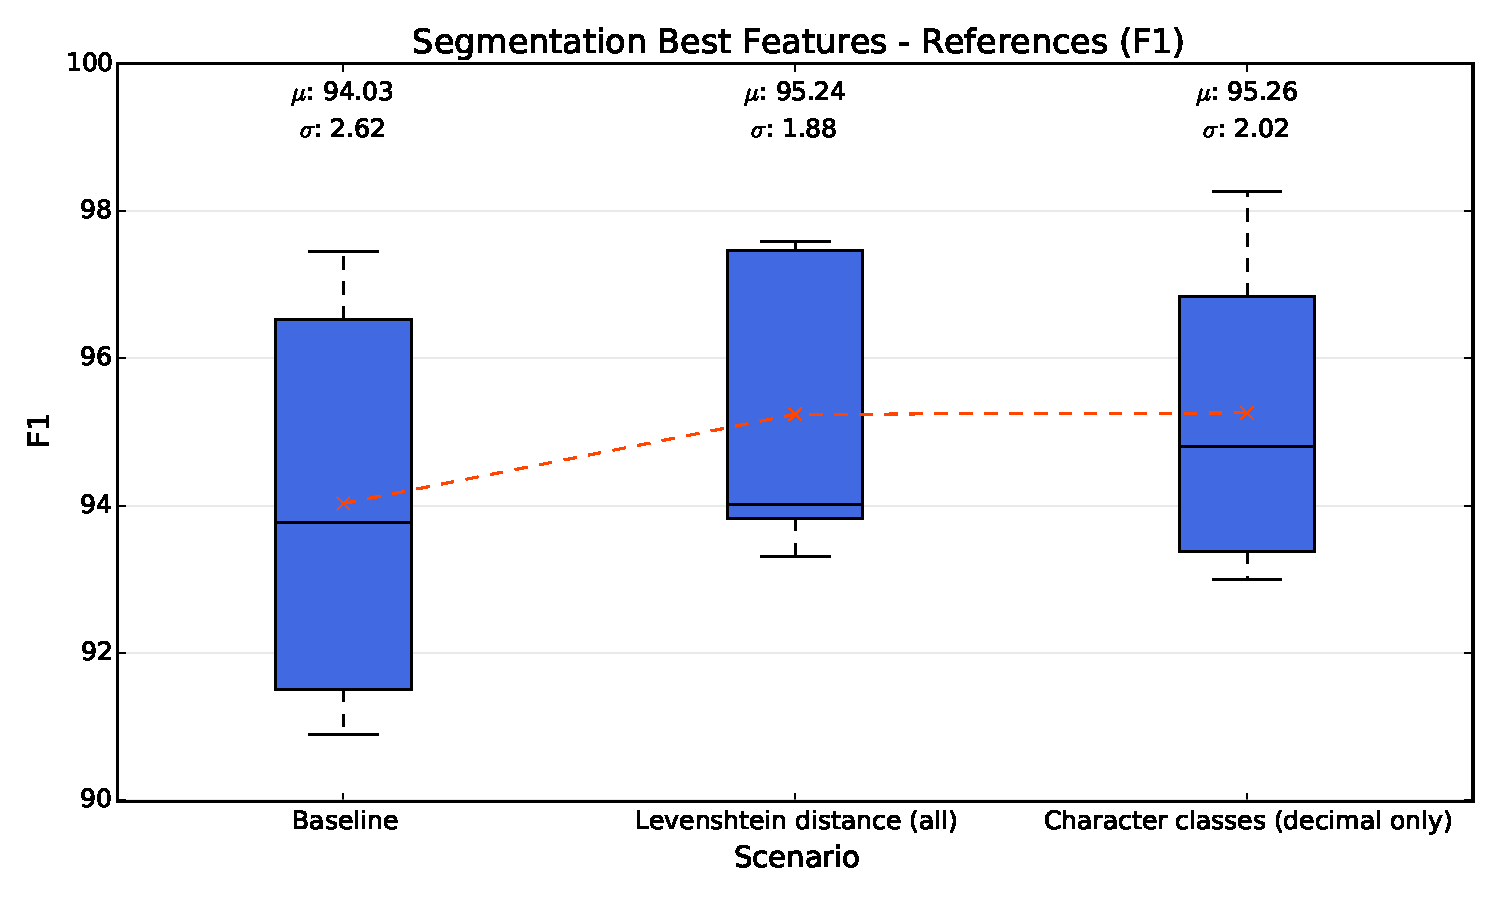
\includegraphics[width=5.5in]{Figures/references.pdf}
\caption{Comparison of baseline, Levenshtein distance and character class features for the reference extraction.}
\label{fig:references}
\end{figure}

The confusion matrix for character classes (decimal only) on HEP papers in Figure \ref{fig:confusion_segmentation} shows a dramatic improvement over the baseline (Figure \ref{fig:confusion_header}). Of particular interest is the increase across the main diagonal, that is true positives (TP) in every class but one, <annex>, where it decreases from 1805 to 1573. Also of interest is the huge reduction (906 to 312) of false negatives for the <header> class to the <body>, explaining where the improvements are being made. Note that this was accompanied by a smaller increase of false positives from <body> to <header> (303 to 530). Another remarkable improvement is the reduction (from 115 to 0) of false positives for the <acknowledgement> class for an expected <references> class. In general, classifications of the <acknowledgement> class improved considerably. Also, <header> lines previously lost to the <cover> page were reduced from 43 to 1.  We may conclude, finally, that though the overall performance of CC was slightly lower than the LD, we should prefer the CC feature variation due to its outstanding performance in key classes, <header> and <references>. In combination, the two features did not yield any additional gains.

\begin{figure}[h]
\center
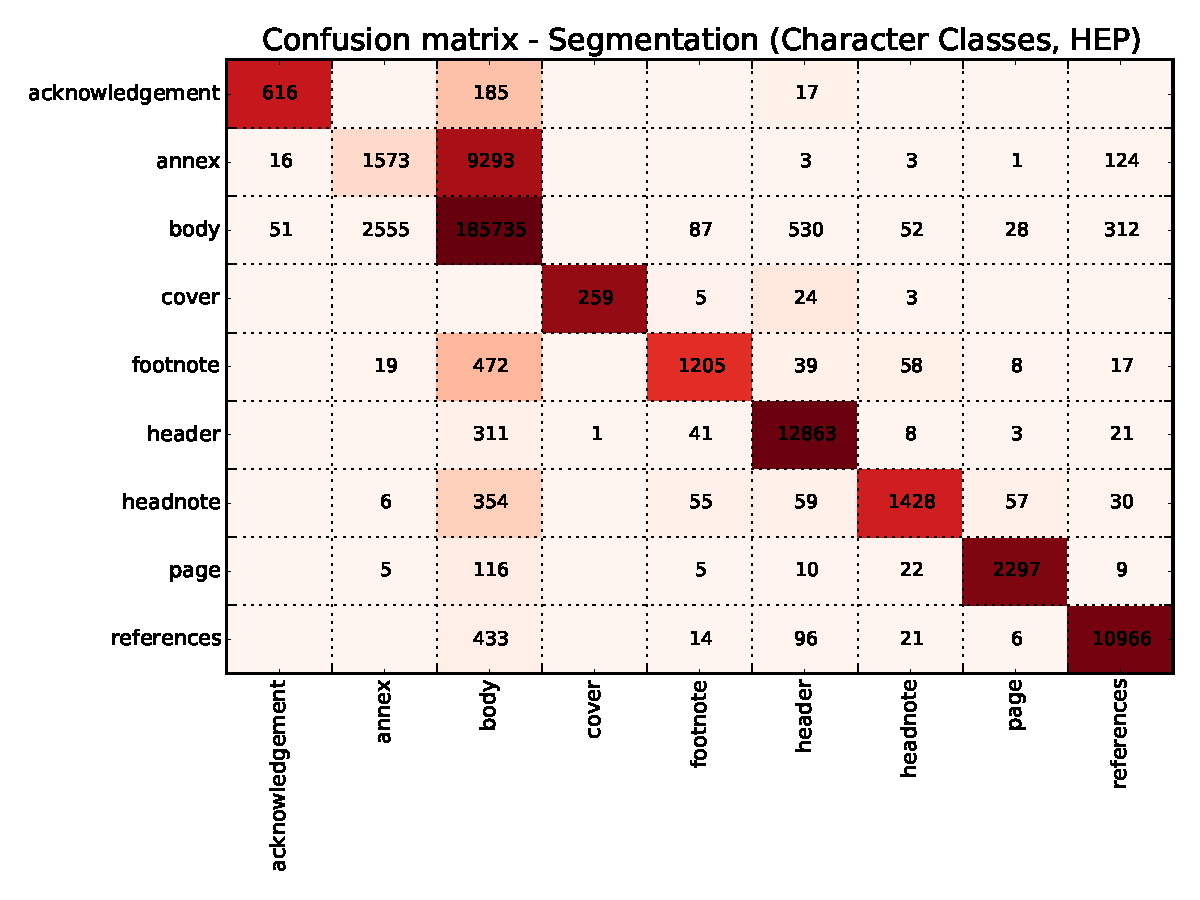
\includegraphics[width=5.5in]{Figures/classes_confusion_segmentation.pdf}
\caption{Confusion matrix for segmentation model with character class features, trained on the pure HEP dataset. Counts are given, as well as a heatmap to indicate the most frequent classifications.}
\label{fig:confusion_segmentation}
\end{figure}


